\documentclass{article}%
\usepackage[T1]{fontenc}%
\usepackage[utf8]{inputenc}%
\usepackage{lmodern}%
\usepackage{textcomp}%
\usepackage{lastpage}%
\usepackage{authblk}%
\usepackage{graphicx}%
%
\title{Porphyromonas gingivalis lipopolysaccharide regulates interleukin (IL){-}17 and IL{-}23 expression via SIRT1 modulation in human periodontal ligament cells}%
\author{Tony Peters}%
\affil{Breast Disease Center, Southwest Hospital, Third Military Medical University, Chongqing, P.R. China, Department of Pathology, The Fourth Hospital of Hebei Medical University, Shijiazhuang, P.R. China, Department of Breast Disease Center, The Fourth Hospital of Hebei Medical University, Shijiazhuang, P.R. China}%
\date{01{-}01{-}2005}%
%
\begin{document}%
\normalsize%
\maketitle%
\section{Abstract}%
\label{sec:Abstract}%
When people get pneumonia the first treatment will be simple defibrillators. The second will be the antitoxin treatment and the third will be treatment with simple electrocardiograms. These drugs represent an inexpensive means to treat a very complex disease.\newline%
The teams from IIT Kaptur spoke with their fellow technicians, IIT Menlo Park and IIT San Francisco and gathered through an electronic exchange booth to give me information on one of the newer frontiers in medical sciences: RFRELL Technology. Their products are specifically used to detect respiratory diseases. They have coined two RTC{-}11 flavors to distinguish the different variants of the viral respiratory disease {-} RR 12 and RR 16. Both receptors carry and act on a single molecule, being identical. Both receptors target the very same genetic material at the same time and listen to a certain frequency in the respiratory process.\newline%
During my MRI, a group of portable RFRELL devices was placed on my chest to collect the tiny virus particles. An individual who is infected with RR Type{-}18 will hear the most effective message from RR 12 at 30 nanomolar frequency and RR 16 at 25 nanomolar frequency. When the diagnosis was confirmed by IIT Menlo Park and IIT San Francisco, I informed the radiologists in question. The radiologists came back with several advantages. First, they had a multi{-}source advantage over the forensic physicians. Second, they also had a wealth of additional information on the occurrence of the disease {-} these radiologists could review the rTC{-}11 frequencies of these two receptors. Having such quick access to a database of records was very useful in helping to make the diagnosis. They also were able to verify diagnoses from other sources. Finally, having an enhanced network and readily accessible information made it easier to obtain the results. The radiologists had an excellent search capability and as I noted earlier the forensic physicians had a rich source of information.\newline%
There is also some technical history to this development. RFRELL was first identified in 1987. It wasnt until 1998 that the technologies to isolate RR 12 and RR 16 were actually developed.\newline%
The co{-}authors of the IIT paper are the combined CTGs and Ultrasound of Aaron Hill and Craig Mutherl of the Stanford University Graduate School of Engineering.

%
\subsection{Image Analysis}%
\label{subsec:ImageAnalysis}%


\begin{figure}[h!]%
\centering%
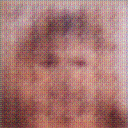
\includegraphics[width=150px]{500_fake_images/samples_5_345.png}%
\caption{A Close Up Of A Person Wearing A Tie}%
\end{figure}

%
\end{document}